\documentclass[11pt,a4paper]{article}
\usepackage[utf8]{inputenc}
\usepackage[vietnamese]{babel}
\usepackage{amsmath,amssymb}
\usepackage[version=4]{mhchem}
\usepackage{geometry}
\geometry{top=1.5cm,bottom=1.2cm,left=1.4cm,right=1.4cm,headheight=28pt,headsep=12pt,footskip=18pt}
\usepackage{graphicx}
\usepackage{xcolor}
\usepackage{tabularx}
\usepackage{array}
\usepackage{tikz}
\usepackage{multicol}
\usepackage{fancyhdr}
\usepackage{enumitem}

\definecolor{hfRed}{HTML}{D32F2F}
\definecolor{hfGreen}{HTML}{8BC390}
\definecolor{mainGreen}{HTML}{2E7D32}

\usepackage{ex_test}
\bracketExpl{true}

\pagestyle{fancy}
\fancyhf{}
\renewcommand{\headrulewidth}{0.75pt}
\renewcommand{\headrule}{\hbox to\headwidth{\color{hfGreen}\leaders\hrule height \headrulewidth\hfill}}
\renewcommand{\footrulewidth}{0.75pt}
\renewcommand{\footrule}{\hbox to\headwidth{\color{hfGreen}\leaders\hrule height \footrulewidth\hfill}}

\fancyhead[L]{\small\itshape\color{hfRed}Tài liệu lưu hành nội bộ}
\fancyhead[R]{\small\color{hfRed}Thầy \textbf{TRẦN VĂN THẠNH} - 0777.470.803}

\fancyfoot[L]{\footnotesize\itshape\color{hfRed}CS1: 6/15 Nguyễn Hoàng, P. Kim Long, TP Huế \quad|\quad CS2: 24 Đặng Thái Thân, TP Huế}
\fancyfoot[R]{\small\textbf{\color{hfRed}Trang \thepage}}

\setlength{\parindent}{0pt}
\setlength{\parskip}{1.8pt}

\def\loigiai#1{}

\begin{document}

\Opensolutionfile{ans}[ans-de09-hs]

\noindent
\begin{minipage}[t]{0.48\textwidth}
	\centering
	\textbf{SỞ GIÁO DỤC VÀ ĐÀO TẠO THỪA THIÊN HUẾ}\\
	\textbf{ĐỀ CHÍNH THỨC}\\
	\textit{(Đề thi có 04 trang)}
\end{minipage}\hfill
\begin{minipage}[t]{0.48\textwidth}
	\centering
	\textbf{\color{mainGreen}ĐỀ KIỂM TRA ĐỊNH KỲ CHƯƠNG 3 (HỢP CHẤT NITROGEN)}\\
	\textbf{MÔN: HOÁ HỌC -- LỚP 12}\\
	\textit{Thời gian làm bài: 50 phút (không kể thời gian phát đề)}\\
	\textbf{Mã đề thi: 109}
\end{minipage}


\vspace{0.1cm}
\noindent\textit{Họ, tên thí sinh: \dots\dots\dots\dots\dots\dots\dots\dots\dots\dots\dots\dots\dots\dots\dots\dots\dots\dots\dots\dots\dots\dots Lớp: \dots\dots\dots\dots SBD: \dots\dots\dots\dots}\\
\noindent\textit{(Cho biết nguyên tử khối: H = 1; C = 12; N = 14; O = 16; Na = 23; S = 32; Cl = 35,5; Fe = 56; Cu = 64).}

\vspace{0.15cm}
\noindent
\textbf{PHẦN I (4,5 điểm -- 18 câu): Câu trắc nghiệm nhiều phương án lựa chọn.}\\
\textit{Thí sinh trả lời từ câu 1 đến câu 18. Mỗi câu hỏi thí sinh chỉ chọn một phương án.}

\setcounter{ex}{0}

\begin{ex}
(SBT -- KNTT). Trong phân tử amine, nguyên tử nitrogen có số cặp electron chưa liên kết là
\choice
{một cặp}
{hai cặp}
{ba cặp}
{không cặp}
\loigiai{}
\end{ex}

\begin{ex}
Cho dung dịch methylamine phản ứng với dung dịch nào sau đây tạo được kết tủa?
\choice
{\ce{NaCl}}
{\ce{Ba(NO3)2}}
{\ce{FeCl3}}
{\ce{K2SO4}}
\loigiai{}
\end{ex}

\begin{ex}
(SBT -- CTST). Phát biểu nào sau đây \textbf{không} đúng về ứng dụng của amine?
\choice
{Các amine đều độc, chủ yếu dùng sản xuất thuốc diệt nấm mốc, kháng sinh}
{Amine được sử dụng nhiều trong bào chế dược phẩm, vitamin}
{Nhiều polymer như nylon-6,6, polyurethane có thể tổng hợp từ amine}
{Phẩm nhuộm azo và dược phẩm là ứng dụng quan trọng của aniline}
\loigiai{}
\end{ex}

\begin{ex}
Số nguyên tử oxygen có trong một phân tử glutamic acid là
\choice
{1}
{3}
{4}
{2}
\loigiai{}
\end{ex}

\begin{ex}
(SBT -- CĐ). Các amino acid tồn tại ở trạng thái ion lưỡng cực, do đó chúng
\choice
{có nhiệt độ nóng chảy cao và tan tốt trong nước}
{có nhiệt độ nóng chảy cao và ít tan trong nước}
{dễ nóng chảy và tan tốt trong nước}
{dễ nóng chảy và ít tan trong nước}
\loigiai{}
\end{ex}

\begin{ex}
Cho phản ứng sau:
\centerline{\ce{H2NCH2COOH + C2H5OH} $\underset{t^\circ}{\overset{\text{HCl}}{\rightleftharpoons}}$ \ce{H2NCH2COOC2H5 + H2O}}\par
Phản ứng trên thể hiện tính chất nào của amino acid cụ thể là glycine?
\choice
{Lưỡng tính}
{Acid mạnh}
{Base mạnh}
{Ester hóa}
\loigiai{}
\end{ex}

\begin{ex}
Biểu diễn dạng kí hiệu của peptide: \ce{HOOC-CH2-NH-CO-CH(CH3)NH2} là:
\choice
{Val-Ala}
{Ala-Val}
{Ala-Gly}
{Gly-Ala}
\loigiai{}
\end{ex}

\begin{ex}
Trong phân tử tetrapeptide Gly-Glu-Ala-Val, amino acid đầu N là
\choice
{Valine}
{Alanine}
{Acid glutamic}
{Glycine}
\loigiai{}
\end{ex}

\begin{ex}
Số gốc $\alpha$-amino acid trong phân tử tripeptide mạch hở là:
\choice
{1}
{3}
{2}
{4}
\loigiai{}
\end{ex}

\begin{ex}
Các protein khác nhau đảm nhận nhiều vai trò thiết yếu khác nhau với sự sống như xây dựng tế bào, xúc tác sinh hoá, điều hoà chuyển hoá chất, vận chuyển chất, kháng thể\dots{} Protein là hợp chất cao phân tử được tạo thành từ một hay nhiều
\choice
{mắc xích}
{chuỗi polypeptide}
{monomer}
{phân tử}
\loigiai{}
\end{ex}

\newpage

\begin{ex}
(SBT -- CTST). Chất có khả năng tạo phức với methylamine và ethylamine trong các chất sau đây là
\choice
{\ce{Ca(OH)2}}
{\ce{Cu(OH)2}}
{\ce{Al(OH)3}}
{\ce{KOH}}
\loigiai{}
\end{ex}

\begin{ex}
(SBT -- CTST). Có bao nhiêu amino acid cần thiết phải cung cấp cho cơ thể thông qua thực phẩm, dinh dưỡng?
\choice
{9}
{20}
{10}
{18}
\loigiai{}
\end{ex}

\begin{ex}
(SBT -- CĐ). Cho các chất có công thức cấu tạo sau:\\
{\centering
	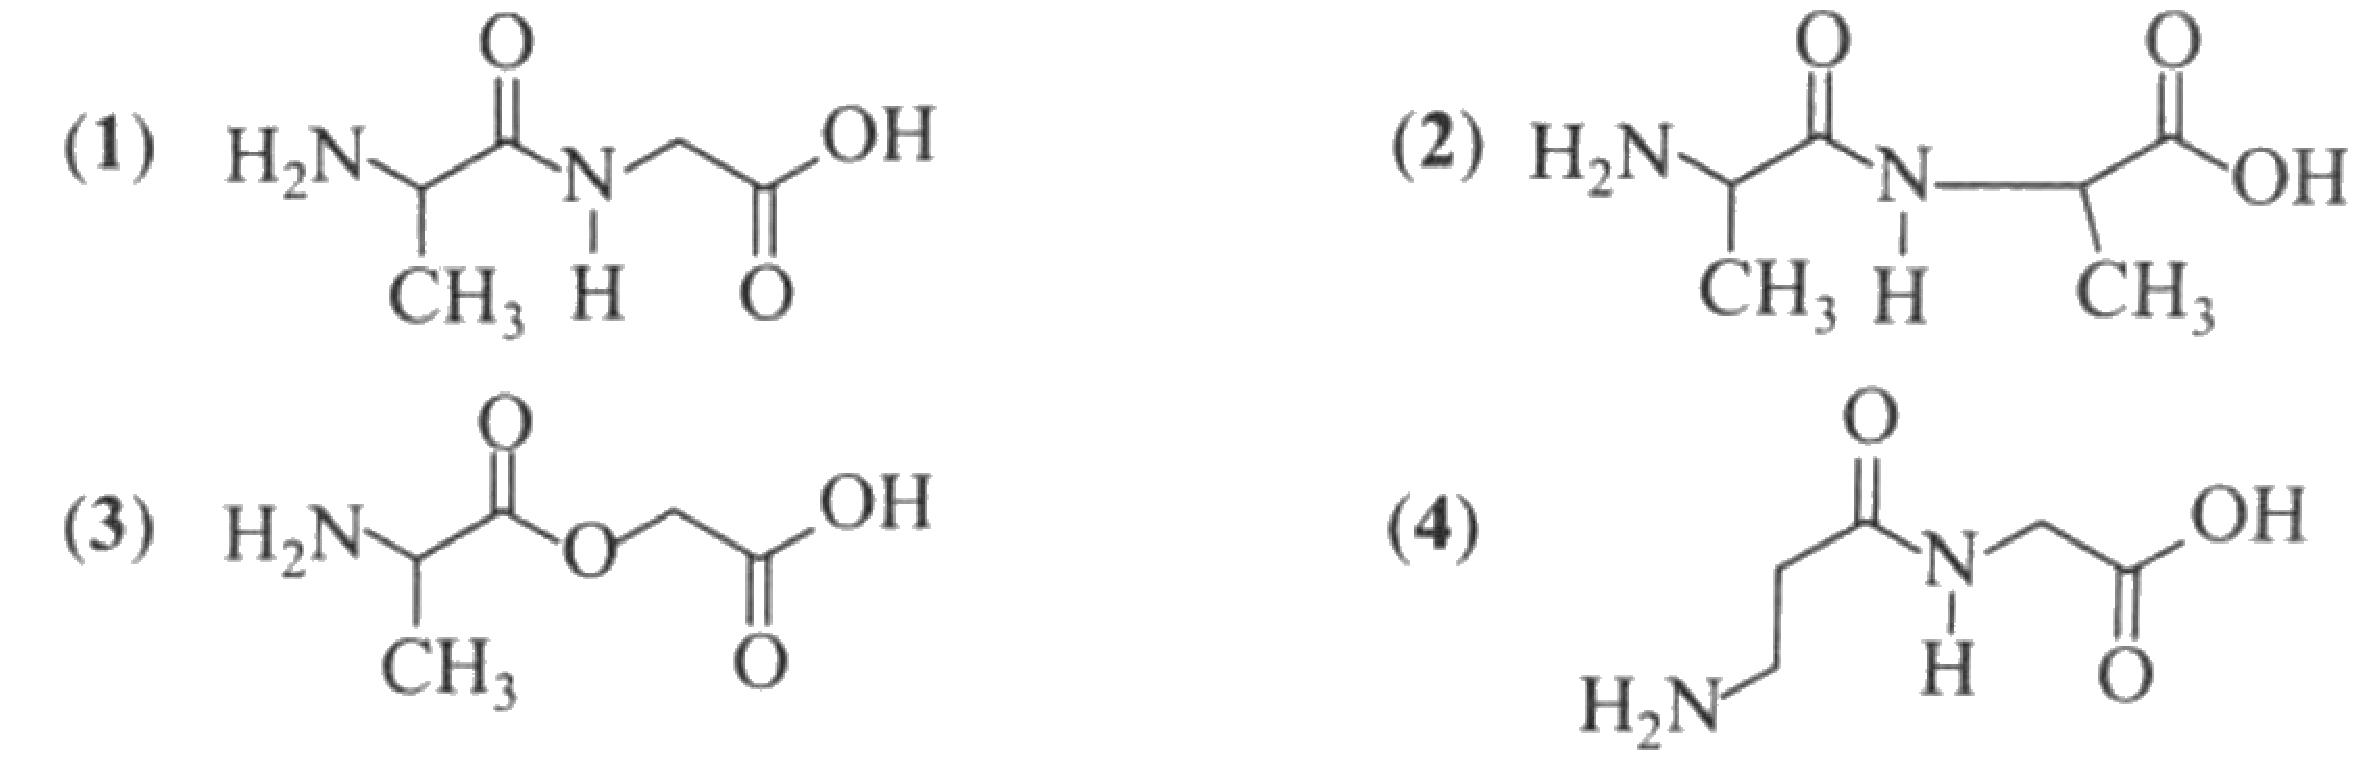
\includegraphics[width=9.5cm]{images_crop_de09/cau13_dipeptides.png}\par}
Trong các hợp chất trên, những hợp chất nào thuộc loại dipeptide?
\choice
{Hợp chất (1) và (2)}
{Hợp chất (1) và (3)}
{Hợp chất (2) và (3)}
{Hợp chất (2) và (4)}
\loigiai{}
\end{ex}

\begin{ex}
(SBT -- CĐ). Trong cấu trúc phân tử của chất cho ở hình bên, liên kết peptide là
{\centering
	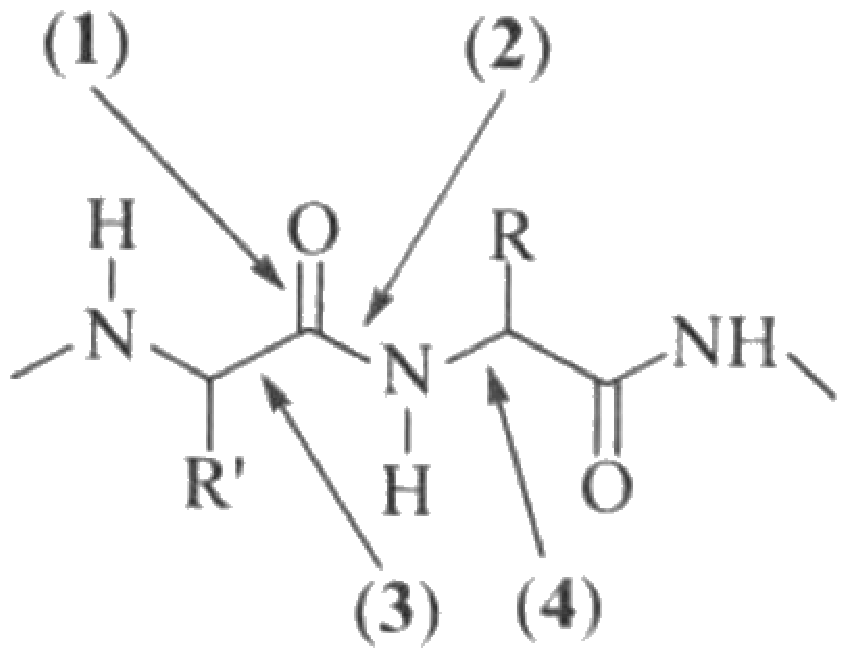
\includegraphics[width=4.5cm]{images_crop_de09/cau14_peptide_bond.png}\par}
\choice
{liên kết (1)}
{liên kết (3)}
{liên kết (2)}
{liên kết (4)}
\loigiai{}
\end{ex}

\begin{ex}
(SBT -- CTST). Loại dinh dưỡng nào sau đây \textbf{không} được cơ thể dự trữ để sử dụng?
\choice
{Tinh bột}
{Chất béo}
{Amino acid}
{Acid béo}
\loigiai{}
\end{ex}

\begin{ex}
(SBT -- CĐ). Cho các hợp chất có công thức cấu tạo dưới đây:
{\centering
	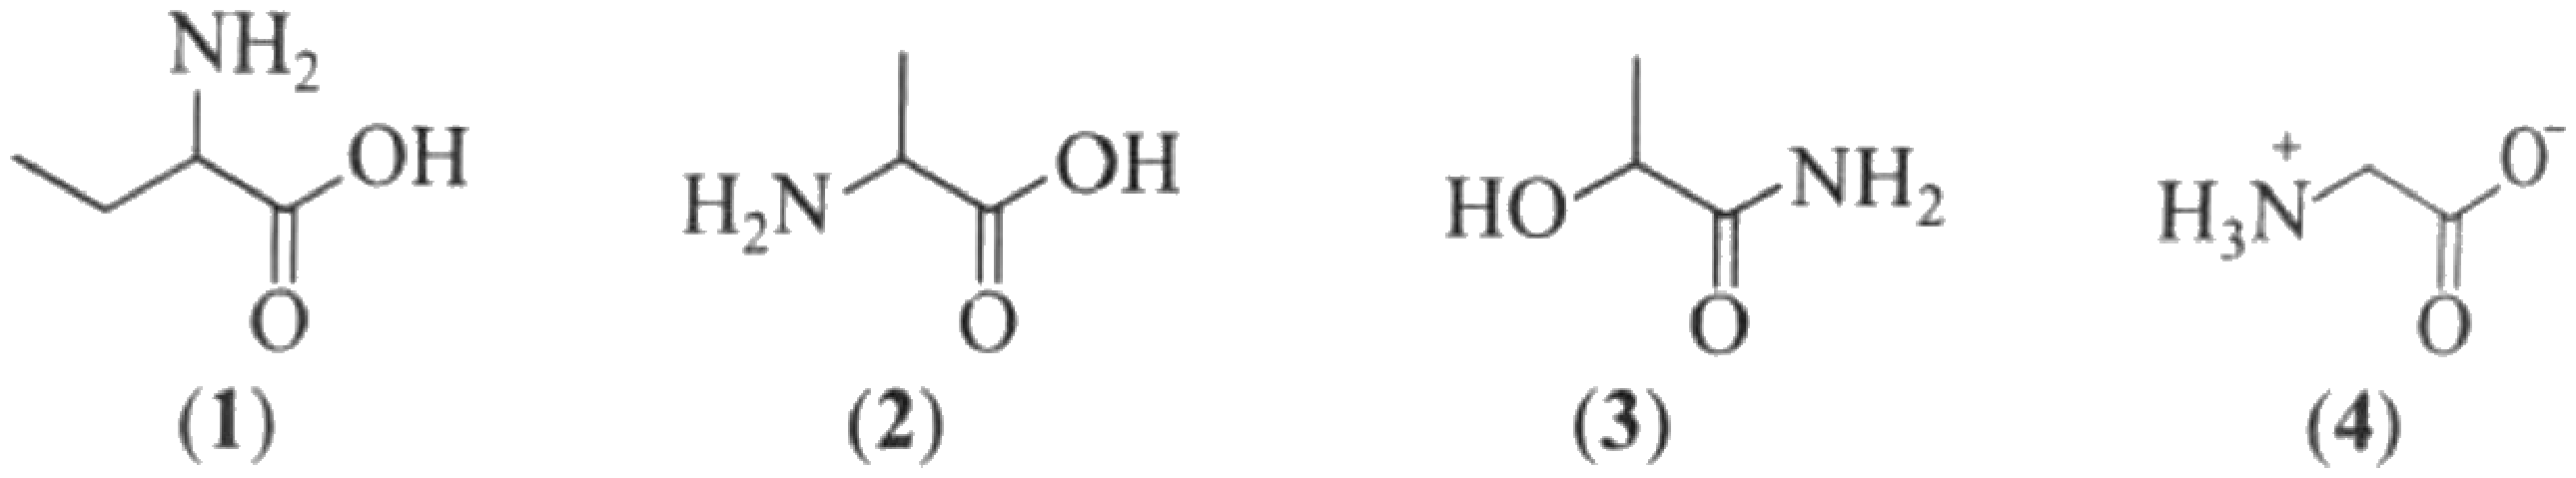
\includegraphics[width=10.0cm]{images_crop_de09/cau16_amino_acids.png}\par}
Những hợp chất nào trong số các chất trên thuộc loại $\alpha$-amino acid?
\choice
{Chất (2), chất (3) và chất (4)}
{Chất (1) và chất (2)}
{Chất (1) và chất (3)}
{Chất (1), chất (2) và chất (4)}
\loigiai{}
\end{ex}

\begin{ex}
(SBT -- CĐ). Chất nào dưới đây \textbf{không} phải là amino acid?
\choice
{Lysine}
{Glycine}
{Aniline}
{Glutamic acid}
\loigiai{}
\end{ex}

\begin{ex}
Cho các phát biểu sau:\\
(a) Sục khí \ce{CH3NH2} vào dung dịch \ce{FeCl3} có sinh ra kết tủa màu xanh.\\
(b) Không thể dùng quỳ tím để phân biệt ba dung dịch: alanine, lysine, glutamic acid.\\
(c) Dung dịch glutamic acid đổi màu quỳ tím thành xanh.\\
(d) Nhỏ vài giọt nước bromine vào dung dịch aniline thu được kết tủa đỏ nâu.\\
(e) Cho dung dịch HCl vào dung dịch glutamic acid thì không có phản ứng xảy ra.\\
(g) Methylamine có lực base yếu hơn ammonia.\\
Số phát biểu đúng là
\choice
{5}
{4}
{0}
{3}
\loigiai{}
\end{ex}

\Closesolutionfile{ans}

\newpage

\vspace{0.15cm}
\noindent
\textbf{PHẦN II (4,0 điểm -- 4 câu): Câu trắc nghiệm đúng sai.}\\
\textit{Thí sinh trả lời từ câu 1 đến câu 4. Trong mỗi ý a), b), c), d) ở mỗi câu, thí sinh chọn đúng hoặc sai.}

\setcounter{ex}{0}

\begin{ex}
(SBT -- KNTT). Các phát biểu về tính chất hoá học của dung dịch methylamine:
\choiceTF
{Phản ứng với HCl tạo thành \ce{CH3NH3Cl}}
{Hoà tan \ce{Cu(OH)2} tạo thành $\ce{[Cu(CH3NH2)4](OH)2}$}
{Phản ứng với \ce{FeCl3} tạo thành kết tủa \ce{Fe(OH)3}}
{Phản ứng với \ce{HNO2} tạo thành $\ce{CH3N2+}$}
\loigiai{}
\end{ex}

\begin{ex}
(SBT -- CTST). Cho một số hợp chất chứa nguyên tố nitrogen như hình bên dưới:\\
{\centering
	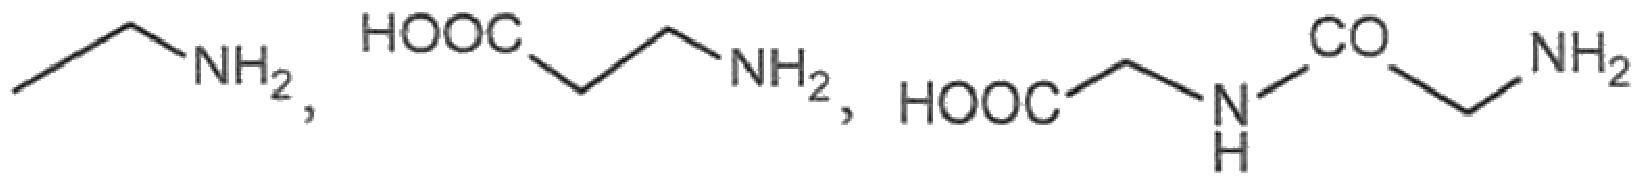
\includegraphics[width=9.5cm]{images_crop_de09/p2_cau2_compounds.png}\par}
Về tính chất vật lí của các chất, xét tính đúng/sai của các phát biểu sau:
\choiceTF
{Dễ tan trong nước}
{Ở điều kiện thường, có 1 chất là chất khí, 1 chất lỏng và 1 chất rắn}
{Chất có nhiệt độ nóng chảy thấp nhất là \ce{CH3CH2NH2}, cao nhất là \ce{HOOCCH2NHCOCH2NH2}}
{Khả năng tan tốt trong nước của các chất là do sự phân cực mạnh trong phân tử}
\loigiai{}
\end{ex}

\begin{ex}
Một peptide có cấu trúc như sau:
{\centering
	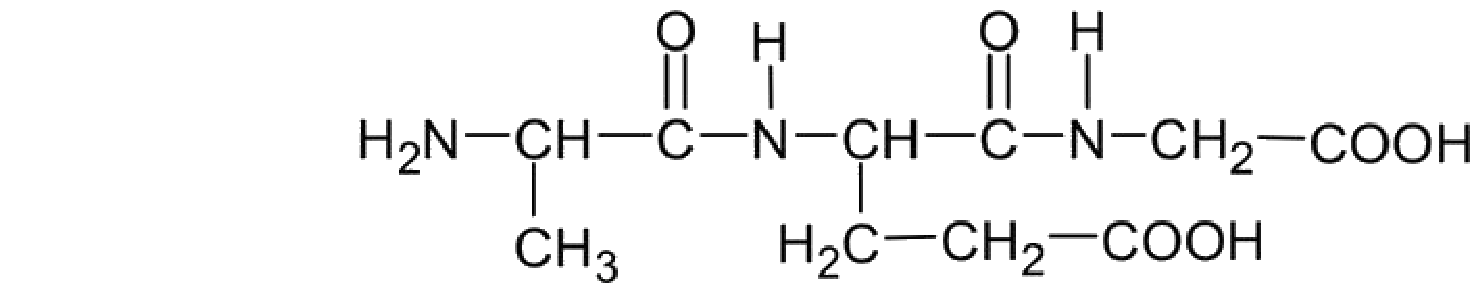
\includegraphics[width=8.5cm]{images_crop_de09/p2_cau3_tripeptide.png}\par}
\choiceTF
{Peptide trên chứa alanine, glutamic acid và glycine}
{Peptide trên có 3 liên kết peptide trong phân tử trên}
{Peptide trên có phản ứng màu biuret}
{Peptide trên là tetrapeptide}
\loigiai{}
\end{ex}

\begin{ex}
Bromelain và papain là những enzyme có tác dụng thuỷ phân protein. Bromelain có nhiều trong quả dứa (thơm). Bromelain được sử dụng để làm thuốc giảm sưng (viêm), điều trị viêm loét đại tràng\dots
{\centering
	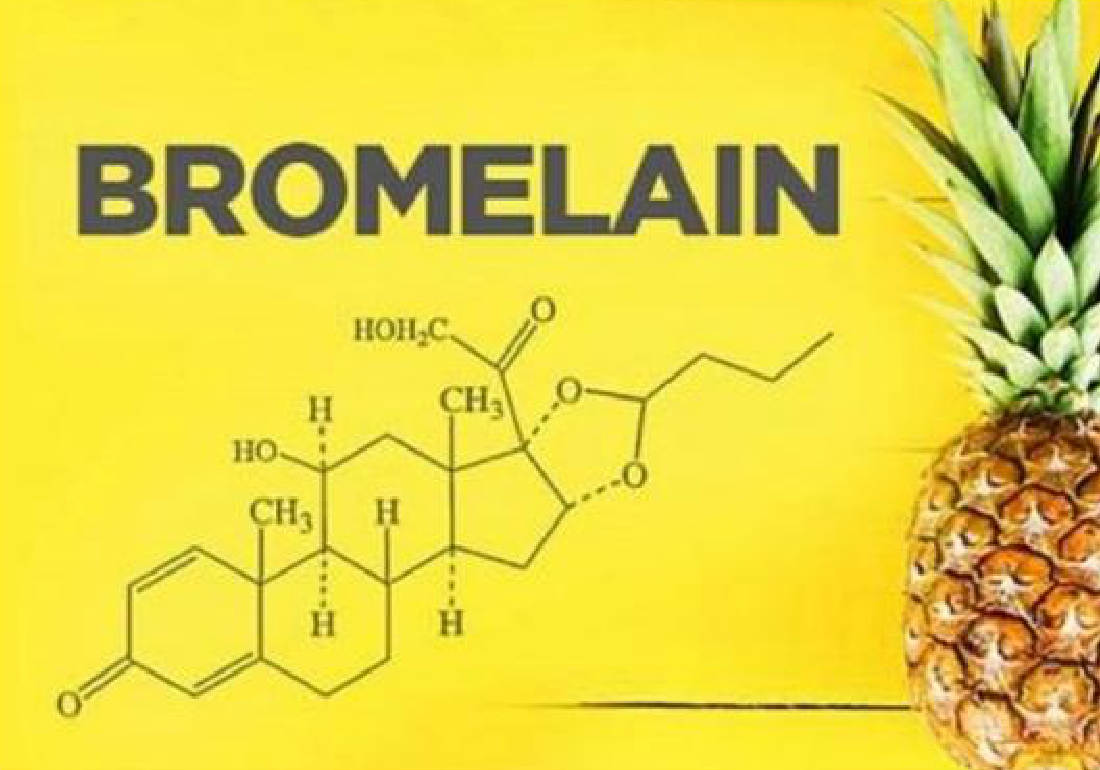
\includegraphics[width=6.0cm]{images_crop_de09/p2_cau4_bromelain.png}\par}
\choiceTF
{Thịt được ướp với nước ép dứa thì khi nấu sẽ nhanh mềm hơn}
{Do enzyme có nhiều trong quả dứa có tác dụng phân giải protein có trong thịt nên khiến cho thịt khi nấu cùng sẽ nhanh mềm hơn}
{Từ dứa có thể chiết xuất được Bromelain}
{Bromelain có chứa 7 nguyên tử oxygen}
\loigiai{}
\end{ex}

\newpage

\vspace{0.15cm}
\noindent
\textbf{PHẦN III (1,5 điểm -- 6 câu): Câu trắc nghiệm yêu cầu trả lời ngắn.}\\
\textit{Thí sinh trả lời từ câu 1 đến câu 6. Mỗi câu hỏi thí sinh điền câu trả lời vào ô tương ứng.}

\setcounter{ex}{0}

\begin{ex}
(SBT -- CTST). Các amine có tính base nên dễ phản ứng với dung dịch acid. Khi cho 1 mol methylenediamine phản ứng với dung dịch acid \ce{HCl} dư, số mol \ce{HCl} tham gia phản ứng là bao nhiêu?
\loigiai{}
\end{ex}
\noindent\textit{Đáp số:} \dotfill\vspace{0.25cm}

\begin{ex}
Trong các dung dịch: \ce{CH3-CH2-NH2}, \ce{H2N-CH2-COOH}, \ce{H2N-CH2-CH(NH2)-COOH}, \ce{HOOC-CH2-CH2-CH(NH2)-COOH}, số dung dịch làm xanh quỳ tím là
\loigiai{}
\end{ex}
\noindent\textit{Đáp số:} \dotfill\vspace{0.25cm}

\begin{ex}
(SBT -- CTST). Cho giá trị nhiệt độ nóng chảy ($^\circ$C) của glycine, trilaurin, \ce{H2O}, aniline, tristearin không theo thứ tự như sau: 0; $-6{,}0$; 46,5; 71,6; 262,0. Giá trị nào phù hợp với nhiệt độ nóng chảy của glycine?
\loigiai{}
\end{ex}
\noindent\textit{Đáp số:} \dotfill\vspace{0.25cm}

\begin{ex}
Cho một số hiện tượng thí nghiệm:\\
(1) Đun nóng dung dịch lòng trắng trứng thấy hiện tượng đông tụ lại, tách ra khỏi dung dịch.\\
(2) Trộn lẫn lòng trắng trứng, dung dịch \ce{NaOH} và một ít \ce{CuSO4} thấy xuất hiện màu đỏ gạch đặc trưng.\\
(3) Nhỏ vài giọt dung dịch \ce{HNO3} đặc vào dung dịch lòng trắng trứng thấy kết tủa màu vàng.\\
(4) Đốt cháy một mẫu lòng trắng trứng thấy xuất hiện mùi khét như mùi tóc cháy.\\
(5) Vắt chanh vào một cốc sữa, ta thấy hiện tượng đông tụ protein xuất hiện.\\
Có bao nhiêu hiện tượng thí nghiệm mô tả đúng?
\loigiai{}
\end{ex}
\noindent\textit{Đáp số:} \dotfill\vspace{0.25cm}

\begin{ex}
Cho một loại protein chứa 3,2\% sulfur về khối lượng. Giả sử trong phân tử chỉ chứa 2 nguyên tử sulfur, phân tử khối của loại protein đó là bao nhiêu?
\loigiai{}
\end{ex}
\noindent\textit{Đáp số:} \dotfill\vspace{0.25cm}

\begin{ex}
Thủy phân hoàn toàn 200 gam hỗn hợp gồm tơ tằm và lông cừu thu được 31,7 g glycine. Phần trăm khối lượng của glycine trong tơ tằm và lông cừu tương ứng là 43,6\% và 6,6\%. Thành phần phần trăm khối lượng tương ứng của tơ tằm trong hỗn hợp ban đầu là a\%. Xác định giá trị của a.
\loigiai{}
\end{ex}
\noindent\textit{Đáp số:} \dotfill\vspace{0.25cm}

\vspace{0.1cm}
\begin{center}
	\textbf{---------- HẾT ----------}
\end{center}

\end{document}
